\FloatBarrier
\section{Testing Strategy}

The first version was validated with 15 manual functional tests. As the system grew to fourteen route modules and twenty-one tables, manual testing could no longer give confidence that a change in one module did not break another. The second phase therefore introduced an automated test suite organised as a test pyramid \cite{cohn2009} (Figure~\ref{fig:pyramid}): many fast unit tests for business rules, a smaller number of integration tests that exercise real HTTP routes against a real MySQL database, component tests for the user interface, and a few end-to-end tests that drive a real browser through complete user journeys.

\begin{figure}[H]
\centering
\resizebox{\textwidth}{!}{%
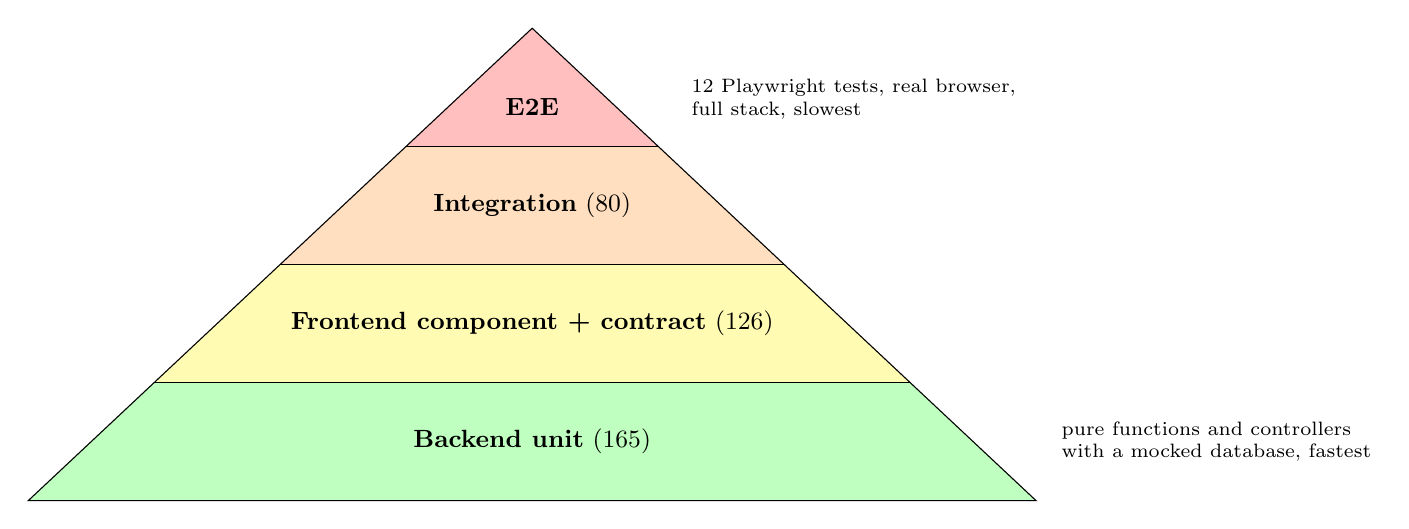
\begin{tikzpicture}[font=\small]
\fill[red!25]    (-1.6,4.5) -- (1.6,4.5) -- (0,6.0) -- cycle;
\fill[orange!25] (-3.2,3.0) -- (3.2,3.0) -- (1.6,4.5) -- (-1.6,4.5) -- cycle;
\fill[yellow!30] (-4.8,1.5) -- (4.8,1.5) -- (3.2,3.0) -- (-3.2,3.0) -- cycle;
\fill[green!25]  (-6.4,0) -- (6.4,0) -- (4.8,1.5) -- (-4.8,1.5) -- cycle;
\draw (-6.4,0) -- (0,6.0) -- (6.4,0) -- cycle;
\draw (-4.8,1.5) -- (4.8,1.5); \draw (-3.2,3.0) -- (3.2,3.0); \draw (-1.6,4.5) -- (1.6,4.5);
\node at (0,5.0) {\textbf{E2E}};
\node[align=center] at (0,3.75) {\textbf{Integration} (80)};
\node[align=center] at (0,2.25) {\textbf{Frontend component + contract} (126)};
\node[align=center] at (0,0.75) {\textbf{Backend unit} (165)};
\node[right, align=left, font=\scriptsize] at (1.9,5.1) {12 Playwright tests, real browser,\\full stack, slowest};
\node[right, align=left, font=\scriptsize] at (6.6,0.75) {pure functions and controllers\\with a mocked database, fastest};
\end{tikzpicture}%
}
\caption{Test Pyramid of Care \& Cure HMS with the Number of Tests at Each Level}
\label{fig:pyramid}
\end{figure}

Three principles guided the tests:
\begin{itemize}
    \item \textbf{Test behaviour, not implementation.} Tests assert on status codes, response bodies, database rows and what the user sees, so that internal refactoring does not break them.
    \item \textbf{Every bug fix gets a regression test} that fails before the fix and passes after it.
    \item \textbf{Tests must be able to fail.} Mutation testing (Section~\ref{sec:mutation}) is used to check that the tests actually detect broken code.
\end{itemize}

\FloatBarrier
\section{Backend Unit Testing}

Unit tests (Jest, 21 files, 165 tests) cover the parts of the backend that contain decisions: the ESI triage function and status transitions, blood compatibility tables and expiry arithmetic, Dijkstra's algorithm, the payment gateway's signature functions, the transaction helper's retry logic, schema-application error filtering, the authentication, validation and error-handling middleware, upload type detection, the JaaS token builder (RS256 signature, room scope, moderator flag), and the bed, bed-request, blood-bank, booking (including the booking limits), emergency, notification, payment and teleconsultation controllers or services. Controllers and services are tested with a mocked database connection, which lets a test assert the exact SQL arguments, the lock order and the error mapping. For example, the bed service test checks that the allocation insert passes \texttt{open\_patient\_id} and \texttt{open\_bed\_id}, that a duplicate-key error on \texttt{uq\_alloc\_open\_bed} becomes ``Bed is not available.'', and that discharge clears both columns.

\FloatBarrier
\section{Backend Integration Testing}

Integration tests (Jest + Supertest, 12 files, 80 tests) send real HTTP requests to the Express application, which talks to a real MySQL database. A setup script creates a separate test database (\texttt{hms\_db\_test}) and applies the same \texttt{schema.sql} and migrations used in production, so the tests also verify that the migrations work. A helper creates a user of any role, logs in, and returns the session and CSRF cookies, so tests exercise the real authentication and CSRF middleware. Each test file creates its own records, removes them afterwards, and closes its database pool and Redis client so that Jest exits cleanly. Rebuilding the test database also flushes its Redis cache index, because a fresh database reuses ids and a stale cached slot list once made a cache test fail about one run in three. Each test file starts one server bound to \texttt{127.0.0.1}: on macOS, letting Supertest listen on all interfaces could pick a port another local application held on \texttt{127.0.0.1}, and requests then reached that application and returned stray \texttt{404} responses.

The integration tests concentrate on what unit tests cannot show: role enforcement on every route (401 for anonymous users, 403 for the wrong role, 404 for other users' records), validation errors, complete workflows (donor $\rightarrow$ donation $\rightarrow$ request $\rightarrow$ fulfil; bed request $\rightarrow$ assign $\rightarrow$ discharge request $\rightarrow$ discharge; order $\rightarrow$ verify $\rightarrow$ paid; paid visit $\rightarrow$ cancel $\rightarrow$ refund due), the hardening rules from two code audits (private prescription files, upload content checks, booking window and limits, slot cleanup, login limits, security headers), and concurrency. Concurrency tests start two conflicting requests at the same time with \texttt{Promise.all} and assert that exactly one succeeds and the other receives \texttt{409}, never a \texttt{500}:

\begin{lstlisting}[language=JavaScript, caption=Concurrency Test for Bed Allocation (beds.routes.test.js)]
test('concurrent allocations of one patient to two beds: one 201, one 409, no 500',
  async () => {
    const [x, y] = await Promise.all([allocate(bedC, p3), allocate(bedD, p3)]);
    expect([x.status, y.status].sort()).toEqual([201, 409]);
  });
\end{lstlisting}

Another test bypasses the application entirely and inserts duplicate open allocations with raw SQL, proving that the database unique keys reject them.

\FloatBarrier
\section{Frontend Component and Contract Testing}

Frontend tests (Vitest + React Testing Library, 19 files, 126 tests) render pages and components in a simulated browser and interact with them the way a user would: typing, clicking and reading visible text. They cover the bed board (including the Allocate dialog that offers pending requests and the highlighted discharge requests), blood bank, emergency board (including the live ESI suggestion and the doctor's \emph{Request bed}), teleconsultation room (payment-required, outside-window and waiting-room states, and the doctor's \emph{Admit}), the per-role layout guard, the admin patient list pager, navigation page, notification bell, patient picker, admin payments pager, patient history (\emph{Pay} button shown only when \texttt{can\_pay} is true), and the MediBot Markdown renderer, including the cross-site scripting payloads described in Chapter~\ref{ch:impl}.

A table-driven \emph{contract test} calls every function of the frontend service layer (more than forty calls across seven services) with a mocked Axios instance and checks the HTTP method, URL and body or query parameters. It catches the most common integration bug in a single-page application, a frontend calling a URL or sending a field name that the backend does not expect, without starting the server.

\FloatBarrier
\section{End-to-End Testing}

End-to-end tests (Playwright, 9 files, 12 tests) start the real backend against the test database and the real frontend, and drive Google Chrome through complete journeys across roles. A global setup step seeds the users and data each journey needs. Table~\ref{tab:e2e} lists the journeys.

\begin{table}[H]
\centering
\caption{End-to-End Test Journeys}
\label{tab:e2e}
\renewcommand{\arraystretch}{1.2}
\begin{tabular}{|L{3.2cm}|L{10.3cm}|}
\hline
\rowcolor{blue!12}
\textbf{Spec} & \textbf{Journey} \\
\hline
beds & Admin allocates a bed to a patient, then discharges it \\
\hline
bed-requests & Doctor requests a bed; admin assigns it; doctor sees the bed and requests the discharge; admin approves it from the highlighted bed \\
\hline
blood-bank & Admin adds a donor, records a donation, then fulfils a request from that stock \\
\hline
emergency & Doctor triages an ESI-1 arrival to the top of the queue, admin is alerted, doctor requests a bed, admin assigns it and the case is admitted \\
\hline
navigation & Visitor routes from Main Entrance to Neurology; the accessible route avoids stairs \\
\hline
notifications-booking & Patient books a video appointment for tomorrow and receives an ``Appointment booked'' notification \\
\hline
payments & Patient pays from history through the mock gateway and the admin sees the payment in the ledger \\
\hline
teleconsult & An unpaid video visit asks for payment; a paid patient waits until the doctor admits them, then both are in the call (the video script is stubbed) \\
\hline
smoke (4 tests) & Every public page, and every page of the patient, doctor and admin portals, renders without console errors, failed API calls or error banners \\
\hline
\end{tabular}
\end{table}

\FloatBarrier
\section{Mutation Testing}
\label{sec:mutation}

A test suite that always passes is not necessarily a good one; it may simply not check the right things. Mutation testing measures this by deliberately introducing small faults (\emph{mutants}) into the code, such as inverting a condition or removing a check, and running the tests: a good suite fails, which ``kills'' the mutant \cite{jia2011}. During the code review of the new modules, twelve hand-written mutants were applied to security- and money-critical code (ownership checks, signature verification, the join window, the past-appointment check, lock guards and others). Eleven were killed immediately. The surviving mutant removed the ownership check on the endpoint that marks a payment order as failed: the existing test only checked that another patient received \texttt{404}, which was still true by accident. A new assertion was added to check that the other patient's request leaves the order untouched in the database, which kills the mutant. A further mutant reverting the MediBot link filter to its earlier regular expression confirmed that the protocol-relative test case (\texttt{/\textbackslash evil.com}) catches the regression.

\FloatBarrier
\section{Code Review Process}

Every change was developed on a feature branch and reviewed before it was merged into \texttt{main} through a pull request. Reviews followed five axes (correctness, readability, architecture, security and performance) and labelled each finding by severity: \textbf{blocker} (must be fixed before merge, e.g. a security hole or data loss), \textbf{major} (a real bug or a missing test), or \textbf{nit} (style or minor clarity). For each module, the reviewer's findings were fixed and the change re-reviewed, with at most two review rounds before remaining findings were either fixed or explicitly recorded. After the system was deployed, two complete code audits of the repository were carried out, each followed by a fix commit with tests; their findings are defects D11--D20 in Table~\ref{tab:defects}. Commit messages describe what changed and why, for example ``Stop payment for past appointments and page the admin payments list'' or ``Escape chatbot messages before rendering them as HTML'', so that the history explains itself.

\FloatBarrier
\section{Continuous Integration}

GitHub Actions runs the pipeline in Figure~\ref{fig:ci} on every push and on every pull request to \texttt{main}. Pull requests in this phase were merged only after all jobs had passed.

\begin{figure}[H]
\centering
\resizebox{\textwidth}{!}{%
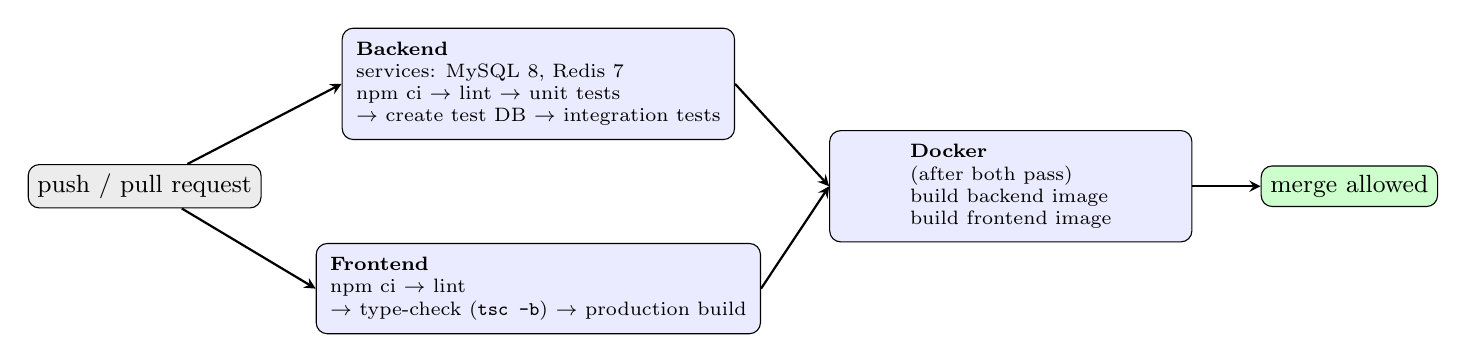
\begin{tikzpicture}[
  job/.style={draw, rounded corners, fill=blue!8, minimum width=4.6cm, align=left, font=\scriptsize, inner sep=5pt},
  arr/.style={->, >=stealth, thick}
]
\node[draw, fill=gray!15, rounded corners, font=\small] (push) at (0,0) {push / pull request};
\node[job] (be) at (5,1.3) {\textbf{Backend}\\services: MySQL 8, Redis 7\\npm ci $\rightarrow$ lint $\rightarrow$ unit tests\\$\rightarrow$ create test DB $\rightarrow$ integration tests};
\node[job] (fe) at (5,-1.3) {\textbf{Frontend}\\npm ci $\rightarrow$ lint\\$\rightarrow$ type-check (\texttt{tsc -b}) $\rightarrow$ production build};
\node[job] (dk) at (11,0) {\textbf{Docker}\\(after both pass)\\build backend image\\build frontend image};
\node[draw, fill=green!20, rounded corners, font=\small] (ok) at (15.3,0) {merge allowed};
\draw[arr] (push) -- (be.west);
\draw[arr] (push) -- (fe.west);
\draw[arr] (be.east) -- (dk.west);
\draw[arr] (fe.east) -- (dk.west);
\draw[arr] (dk) -- (ok);
\end{tikzpicture}%
}
\caption{Continuous Integration Pipeline (GitHub Actions)}
\label{fig:ci}
\end{figure}

The backend job runs the full unit and integration suites against real MySQL and Redis service containers, so the integration test that needs Redis also runs there. At present the frontend job lints, type-checks and builds the application; the Vitest and Playwright suites are run locally before each pull request. Adding them to the pipeline is listed as future work.

\FloatBarrier
\section{Test Results}

Table~\ref{tab:testsummary} in Chapter~\ref{ch:impl} summarises the results: all 165 backend unit tests, all 126 frontend tests, all 80 integration tests and all 12 end-to-end tests pass. ESLint reports no errors in either project, and the TypeScript compiler reports no type errors.

\FloatBarrier
\section{Defects Found and Fixed}

Table~\ref{tab:defects} lists the most significant defects found by the tests, reviews and mutation testing during this phase, and how each was fixed. Each fix is accompanied by a regression test.

\begin{longtable}{|C{0.8cm}|L{4.3cm}|L{3.9cm}|L{4.2cm}|}
\caption{Significant Defects Found and Fixed} \label{tab:defects} \\
\hline
\rowcolor{blue!12}
\textbf{No.} & \textbf{Defect} & \textbf{Impact} & \textbf{Fix} \\
\hline
\endfirsthead
\hline
\textbf{No.} & \textbf{Defect} & \textbf{Impact} & \textbf{Fix} \\
\hline
\endhead
D1 & MediBot replies were inserted into the page as HTML without escaping & Cross-site scripting through prompt injection & Escaping Markdown renderer with a link-scheme whitelist; protocol-relative \texttt{/\textbackslash host} also blocked \\
\hline
D2 & Payment could be started for an appointment whose time had passed & Patients charged for visits that can no longer happen & Server rejects orders more than 60 minutes after the start; \texttt{can\_pay} flag hides the button \\
\hline
D3 & Admin payments list returned every row & Slow page and large responses as data grows & Validated \texttt{page}/\texttt{limit} with \texttt{LIMIT/OFFSET}, total count and pager \\
\hline
D4 & Only application code prevented a second open bed allocation & A race or future code path could double-book a bed & Unique \texttt{open\_bed\_id} and \texttt{open\_patient\_id} keys; duplicate-key errors mapped to 409 \\
\hline
D5 & Database session ran in UTC while slot times are stored in IST & \texttt{NOW()} comparisons 5.5 hours off on cloud servers & Session time zone pinned to +05:30 on every pooled connection \\
\hline
D6 & \texttt{JOIN ... FOR UPDATE} and locks on missing rows & Deadlocks under concurrent admissions and payments & Split locked and unlocked reads, fixed lock order, deadlock retry in \texttt{inTransaction} \\
\hline
D7 & Test for the payment-fail endpoint did not check ownership effects & A removed ownership check would go unnoticed & Assertion that another patient's request leaves the order unchanged \\
\hline
D8 & Jest did not exit after the integration suite & CI jobs hang until timeout & Each test file closes its database pool and Redis client \\
\hline
D9 & Backend kept running when its port was already in use & Silent failure in development and deployment & Process exits with an error if the port cannot be bound \\
\hline
D10 & Development script depended on an uninstalled tool (nodemon) & \texttt{npm run dev} failed on a fresh clone & Uses Node's built-in \texttt{node --watch} \\
\hline
D11 & Prescription files were public static files under \texttt{/uploads}, typed by file name & Anyone with the URL could read another patient's prescription; files lost on restart & Files stored in MySQL, served only to the patient and doctor, type checked by content \\
\hline
D12 & Cancelling did not free the slot (\texttt{slot\_id} was unique) and three cancel paths differed & Cancelled slots were lost; paid cancellations not flagged & One cancel service; \texttt{active\_slot\_id} unique key; \texttt{refund\_due}; other side notified \\
\hline
D13 & MediBot booked through its own endpoint & Past and blocked slots could be booked from the chat & Chat uses \texttt{/api/\allowbreak appointments/\allowbreak book} and lists only bookable slots \\
\hline
D14 & Blocking a day deleted its slots & The midnight generator recreated them, reopening the day & Slots are marked unavailable instead \\
\hline
D15 & Deleting a user or appointment cascaded to payments & Loss of financial records & \texttt{ON DELETE RESTRICT} and a clear 409 \\
\hline
D16 & Nightly cleanup deleted past free slots that cancelled visits still pointed to & Visit history deleted, or cleanup failed on a paid visit and skipped slot generation & Keep referenced slots; cleanup and generation fail independently \\
\hline
D17 & Two first requests raced for the CSRF cookie, and the cookie ended with the browser & Random 403 errors, and logouts, for returning users & Cookie lives as long as the refresh token; \texttt{CSRF\_INVALID} code; one client retry \\
\hline
D18 & One trusted proxy hop behind Vercel and Render; successful logins counted & All visitors shared one rate-limit bucket: 10 logins per 15 minutes for the whole site & \texttt{TRUST\_PROXY\_HOPS=2}; only failures count; extra per-account limit \\
\hline
D19 & Visits could be completed or prescribed long before they started, and slots created for any date & Wrong records; unbounded slot rows & 15-minute rule; booking and slot window of today plus 13 days \\
\hline
D20 & Admin lists loaded every row and counted on the client & Slow pages and wrong dashboard totals as data grew & Server-side filtering, search, sorting and paging \\
\hline
\end{longtable}
